\subsection{Analisi}

\textit{\textbf{Periodo}: dal 2020-11-16 al 2021-01-18}

L'inizio di questa fase coincide con il primo incontro effettuato dai membri del gruppo e si conclude con la scadenza della Revisione dei Requisiti.

\subsubsection{Attività}

\begin{itemize}
\item \textbf{Analisi capitolati}: vengono discussi e analizzati i capitolati presentati e si cerca una scelta definitiva;
\item \textbf{Individuazione degli strumenti}: si determinano tutti gli strumenti necessari per la realizzazione del progetto, compreso di strumenti per la comunicazione, la documentazione, lo sviluppo e la verifica. Si possono inoltre approfondire le tecnologie necessarie per realizzare il prodotto;
\item \textbf{\NdP{}}: vengono definite tutte le regole che il gruppo dovrà rispettare durante l'intero sviluppo del progetto. Il documento inerente viene redatto dall'\ammProg{};
\item \textbf{\SdF{}}: si individuano tutte le informazioni utili rilevate che hanno portato alla scelta del capitolato e all'esclusione degli altri. Il documento inerente viene redatto dall'\analProg{};
\item \textbf{\AdR{}}: vengono identificati i requisiti necessari per lo sviluppo del prodotto e i casi d'uso che soddisfano i precedenti. Il documento inerente viene redatto dall'\analProg{};
\item \textbf{\PdQ{}}: si individuano i metodi necessari per garantire la qualità del prodotto. Il documento inerente viene redatto dall'\ammProg{};
\item \textbf{\PdP{}}: si individuano i rischi, la pianificazione delle attività e i costi di preventivo e consuntivo; viene inoltre riportato l'organigramma del gruppo. Il documento inerente viene redatto dal \respProg{};
\item \textbf{Glossario}: vengono riportati e definiti i termini presenti nei documenti che possono risultare ambigui. Il documento viene redatto da qualsiasi membro del gruppo;
\item \textbf{Consolidamento}: viene realizzata la presentazione da esporre in sede di Revisione dei Requisiti e si approfondiscono aspetti lacunari riguardo il progetto.
\end{itemize}

\subsubsection{Periodi}

\begin{itemize}
\item \textbf{Periodo 1}: \textit{dal 2020-11-16 al 2020-12-02}. \\
Vengono svolte le attività di analisi dei capitolati e individuazione degli strumenti;
\item \textbf{Periodo 2}: \textit{dal 2020-12-02 al 2020-12-23}. \\
Vengono redatti i documenti di \NdP{} e \SdF{}. Vengono inoltre iniziati i documenti di \PdP{} e Glossario;
\item \textbf{Periodo 3}: \textit{dal 2020-12-23 al 2021-01-11}. \\
Vengono redatti i documenti di \PdQ{} e \AdR{} e completati quelli di \PdP{} e Glossario. Il periodo si conclude con la consegna del materiale relativo alla Revisione dei Requisiti;
\item \textbf{Periodo 4}: \textit{dal 2021-01-11 al 2021-01-18}. \\
Viene svolta l'attività di consolidamento. Il periodo si conclude con la Revisione dei Requisiti.
\end{itemize}

\subsubsection{Diagramma di Gantt}

\begin{figure}[H]
\centering

\centerline{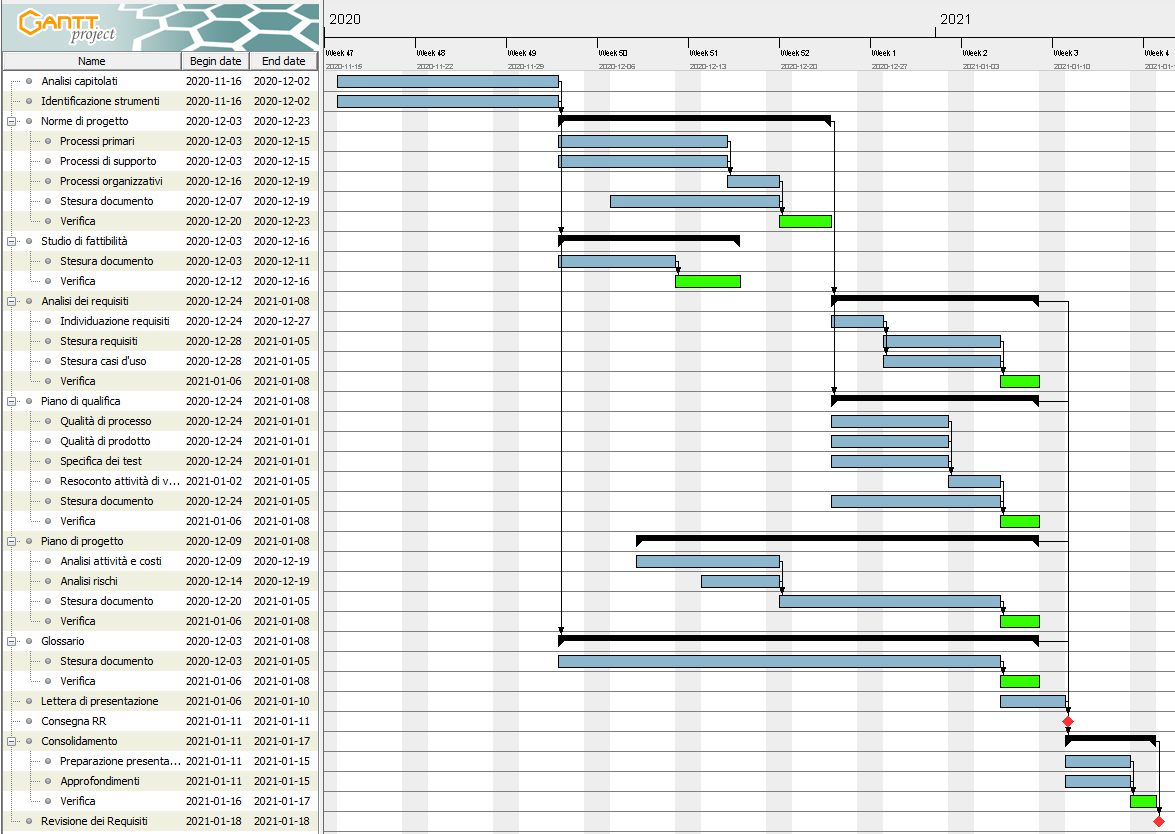
\includegraphics[scale=0.6]{res/Pianificazione/Gantt/analisi}}
\caption{Diagramma di Gantt per il periodo di analisi}
\end{figure}